Como conclusiones finales de este trabajo se logró llevar a la práctica una gran cantidad de los conceptos vistos durante la cursada, a partir del análisis hecho sobre un nuevo modelo se pudo pasar de un sistema resuelto (modelo diferencial) a este que inicialmente resultaba una incógnita. 

A medida que implementamos los distintos componentes necesarios para conseguir el objetivo propuesto adquirimos conocimientos sumamente útiles sobre el sistema bajo estudio, la herramienta de desarrollo y temas anteriormente abordados (cinemática, seguimiento de trayectorias, filtro de kalman), consideramos que el aprendizaje de esto resulta muy enriquecedor 

Centrándonos en los resultados observamos que nuestra implementación presenta buenos resultados y en varias trayectorias no triviales se logró la navegación autónoma dentro del entorno simulado. La experimentación nos permitió ver los atributos que, en su correcta implementación, cada una de las partes partícipes en el sistema (Controlador de posición, seguidor de trayectoria, localizador de Kalman, etc) aportan tanto por separado y funcionando en conjunto.

%Hay algo mas para poner? Como por ejemplo cosas que no habia que hacer pero se pueden mejorar/agregar al TP? 
\pagebreak
\section{Apendice}

\subsection{Detalles del sistema desarrollado}

Para concluir el trabajo presentamos un pantallazo general de todos los nodos trabajando en conjunto:

\begin{figure}[!htb]
\begin{center}
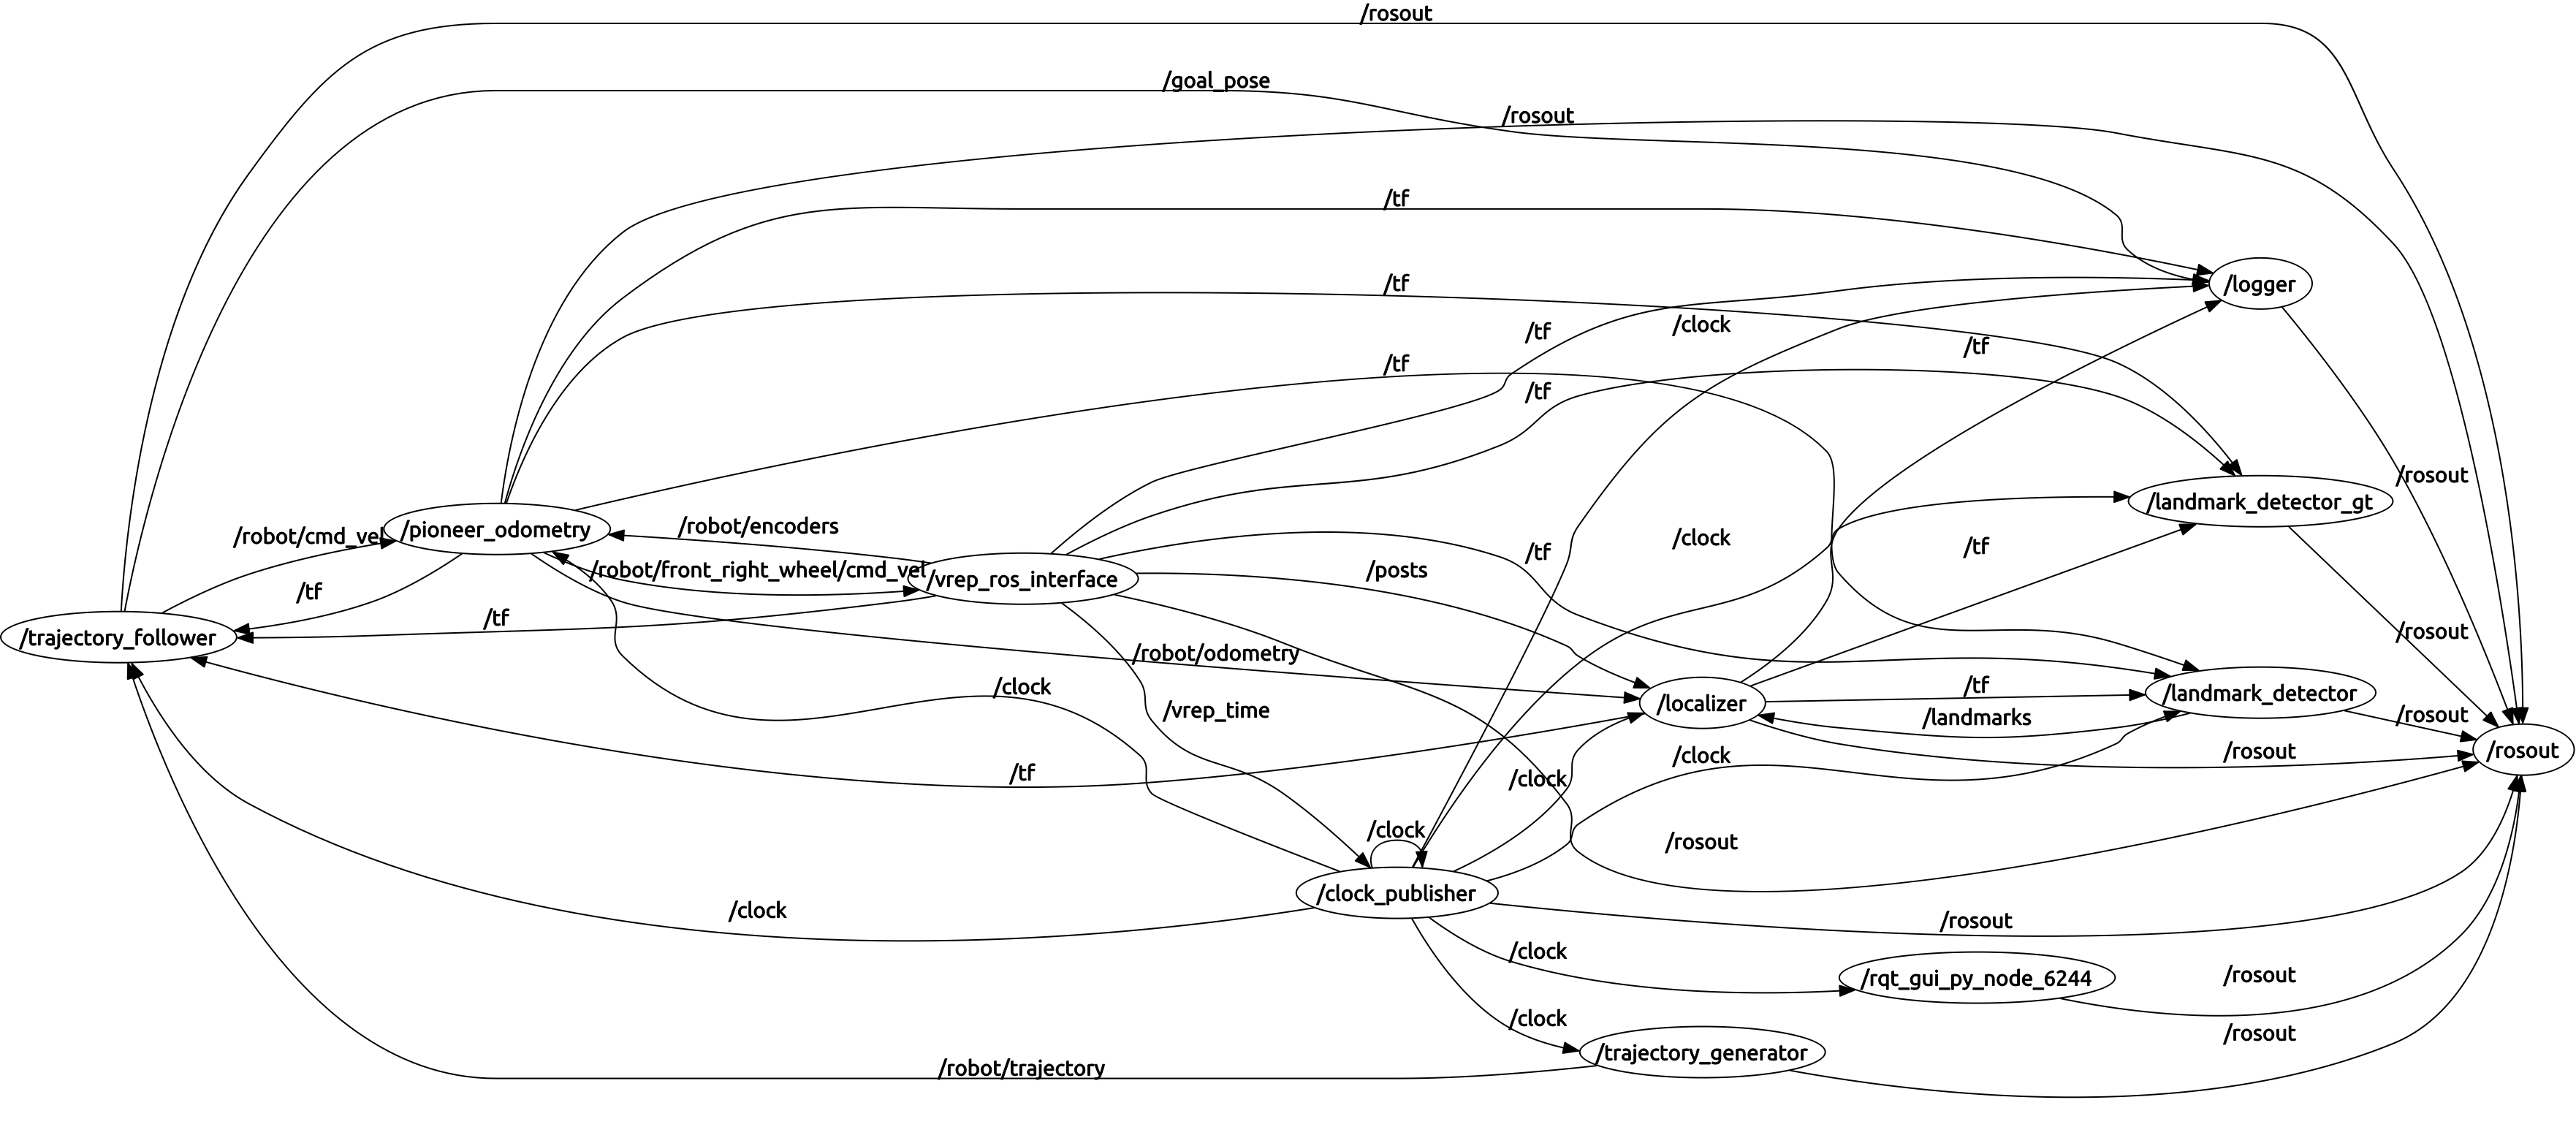
\includegraphics[width=\linewidth]{rqtgraphekf.png} 
\end{center}
\end{figure}

Sobre esta gran cantidad de mensajes siendo intercambiados en paralelo podemos destacar como lo más relevante al problema los siguientes:

El nodo encargado de la odometría recibe la información de los comandos de velocidad t encoders para enviar su estimación de la pose, esta es capturada por el "trajectory follower" que mide la distancia a la pose del goal juntando esto con lo recibido por el "trajectory generator" y publicando las consignas de velocidades necesarias para avanzar hacia el goal.

Por su parte el nodo "localizer" se suscribe a los tópicos de odometría, la información de senado y la ubicación del robot y postes en el simulado, con esto obtiene las consignas de covarianza y publica las transformaciones desde el marco EKF al del robot.

Por último el detector de landmarks de la IMU usa la información usa la información de scanning para actualizar la información de distancia respecto a los "landmarks".